\documentclass[class=minimal, border = 0pt, crop]{standalone}
\usepackage{pgf}
\usepackage{tikz}
\usepackage[utf8]{inputenc}
\usetikzlibrary{arrows,automata,shapes,calc, backgrounds}
\usetikzlibrary{positioning}
\usetikzlibrary{hobby}
\pagestyle{empty}
\newcommand\irregularcircle[2]{% radius, irregularity
  \pgfextra {\pgfmathsetmacro\len{(#1)+rand*(#2)}}
  +(0:\len pt)
  \foreach \a in {10,20,...,350}{
    \pgfextra {\pgfmathsetmacro\len{(#1)+rand*(#2)}}
    -- +(\a:\len pt)
  } -- cycle
}
\begin{document}
\centering
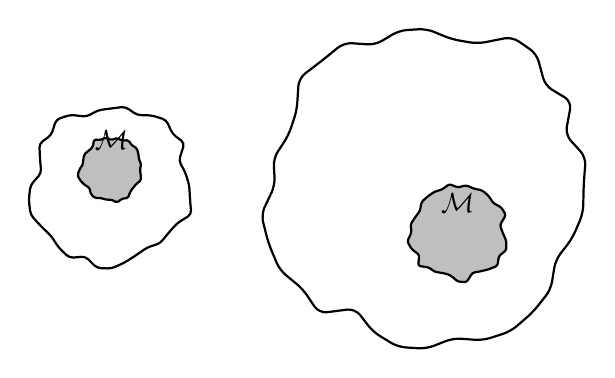
\begin{tikzpicture}
  \coordinate (o1) at (0,0);
  \coordinate (o2) at (-4,0);
  \coordinate (o3) at (0.4,-0.6);
  \coordinate (o4) at (-4,0.2);
  \draw[rounded corners=1mm,thick] (o1) \irregularcircle{2cm}{2mm};
  \draw[rounded corners=0.5mm, thick] (o2) \irregularcircle{1cm}{1mm};
  \draw[rounded corners=0.3mm,thick,fill=gray!50] (o3) \irregularcircle{0.6cm}{0.6mm};
  \draw[rounded corners=0.2mm,thick,fill=gray!50] (o4) \irregularcircle{0.4cm}{0.4mm};
  \node (a1) at (0.4,-0.6) [label=$\mathcal{M}$] {};
  \node (a2) at (-4,0.2) [label=$\mathcal{M}$] {};
\end{tikzpicture}
\end{document}